\section{Results}\label{sec:exp_results}
The TO optimization problems~\eqref{eq::takeoff_opt_prb} and~\eqref{eq::braking_opt_prb} are conveniently written employing the API provided by the Horizon tool~\cite{to::horizon_to} and solved on a 11th Gen Intel(R) Core(TM) i7-11800K CPU, using Ipopt and MA57 linear solver for  step computations. 
The obtained optimal results are then tested both in simulation and on the real hardware.
%showcasing the efficacy of our formulation in capturing the characteristics of the hardware. 
Our leg prototype is based on a 2 DOF
leg prototype the joints of which are actuated by BLDC motor drives with 50:1 gear ratio. The power setup of the
leg makes use of a 25Ah (100A peak discharge current), 51.2V nominal voltage battery unit and the energy flow from and to the battery is measured through a dedicated data acquisition system that monitors the power bus voltage and current levels.
%Convergence plots and additional information on the results are provided in the accompanying video.
\subsection{Take-off generation}
The optimal take-off trajectory is generated solving the TO problem~\eqref{eq::takeoff_opt_prb} with the pipeline described in Sec.~\ref{subsec:takeoff_opt}: first a coarse problem made of $100$ nodes is solved, then the obtained solution is re-sampled~\cite{to::horizon_to} at  $1\mathrm{KHz}$ (corresponding to $917$ nodes for the optimal phase durations found solving~\eqref{eq::takeoff_opt_prb}) and then refined with the same rate and number of nodes, so that a dynamically feasible trajectory is found. The solution of~\eqref{eq::takeoff_opt_prb} is found in $79$ iterations for the coarse initial problem and in $48$ iterations for the refined one (see Fig.~\ref{fig:convergence_plots}). 
Figure~\ref{fig:takeoff_opt_data} shows part of the take-off TO solution and highlights how our formulation is able to exploit the performance of the hardware, while staying inside its limits. 
%For example, looking at the quadrature current, we see that it saturates at the actuator limit of $50\mathrm{A}$ at the take-off instant. Similarly, the actuation torques and joint velocities are close to the peak limit of $120\mathrm{Nm}$ and $20\mathrm{rad/s}$, showing that we are using the hardware close to its peak performance.
\subsection{Landing configuration and landing optimization}\label{sec:land_conf}
As detailed in Section~\ref{subsec:energy_rec_opt}, once a solution of the problem~\eqref{eq:takeoff_opt_L} is available, it is possible to estimate the expected touchdown velocity. In this case, the final tip height is approximately $0.37\mathrm{m}$, for an estimated impact velocity of roughly $2.7\mathrm{m/s}$ (computed as described at the end of Sec.~\ref{subsec:energy_rec_opt}). Using this value as the input to~\eqref{eq::braking_opt_prb}, we solve~\eqref{eq::braking_opt_prb} and obtain the optimal landing impedances and configuration
\begin{eqnarray}\label{eq:optimal_braking_sol}
&K_p^{\mathrm{opt}} = \left[10.65,~23.49\right]~\mathrm{N\,m/rad}\\
&K_d^{\mathrm{opt}} = \left[6.92,~1.67\right]~\mathrm{N\,m/(rad/s)}\\
&\hat{q} = \left[1.34,~1.33\right]~\mathrm{rad}
\end{eqnarray}
after a total of $147$ iterations (see Fig.~\ref{fig:convergence_plots}). Looking at Fig.~\ref{fig:impact_ratio}, the optimal $\hat{q}$ is almost on the same curve of the configurations n.$1$ and n.$2$, with an impact ratio $\rho$ of approximately $3.84~\mathrm{N\,s^{2}/m}$, an impulse $\hat{f}$ of $10.73~\mathrm{N\,s}$ and a total of $37.19~\mathrm{J}$ of theoretical recovered energy.
\begin{figure}[t]
    \centering
    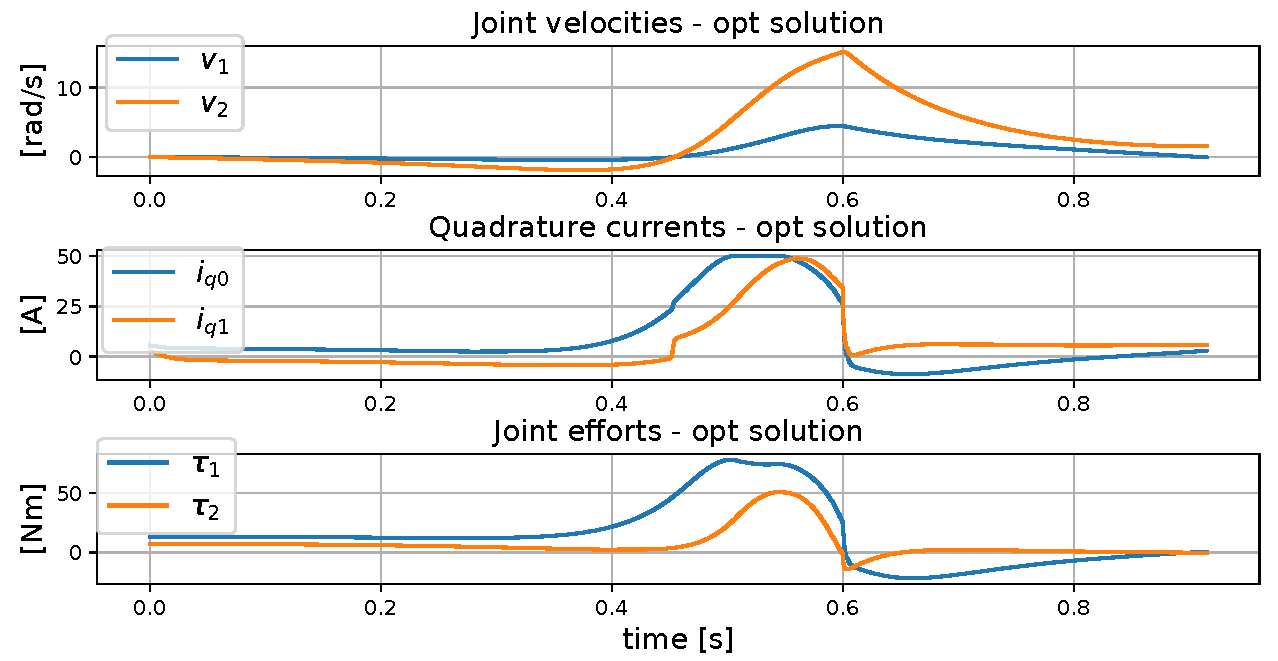
\includegraphics[width=1\columnwidth]{images/hardware_saturation_opt.pdf}
    \caption{Joint velocites, quadrature currents and joint efforts and jump height obtained from the refined take-off trajectory optimization problem. The limits for the quadrature current of $50~\mathrm{A}$ (for safety lower than the maximum peak $i_q$ of $62~\mathrm{A}$ which the control boards can tolerate) are saturated. The peak torque limits of $120~\mathrm{N\,m}$ as well as the maximum link-side velocity of $20~\mathrm{rad/s}$, on the contrary, are not saturated.\vspace{-0.3cm}}
    \label{fig:takeoff_opt_data}
\end{figure}

%\begin{figure}[t]
%	\centering
%	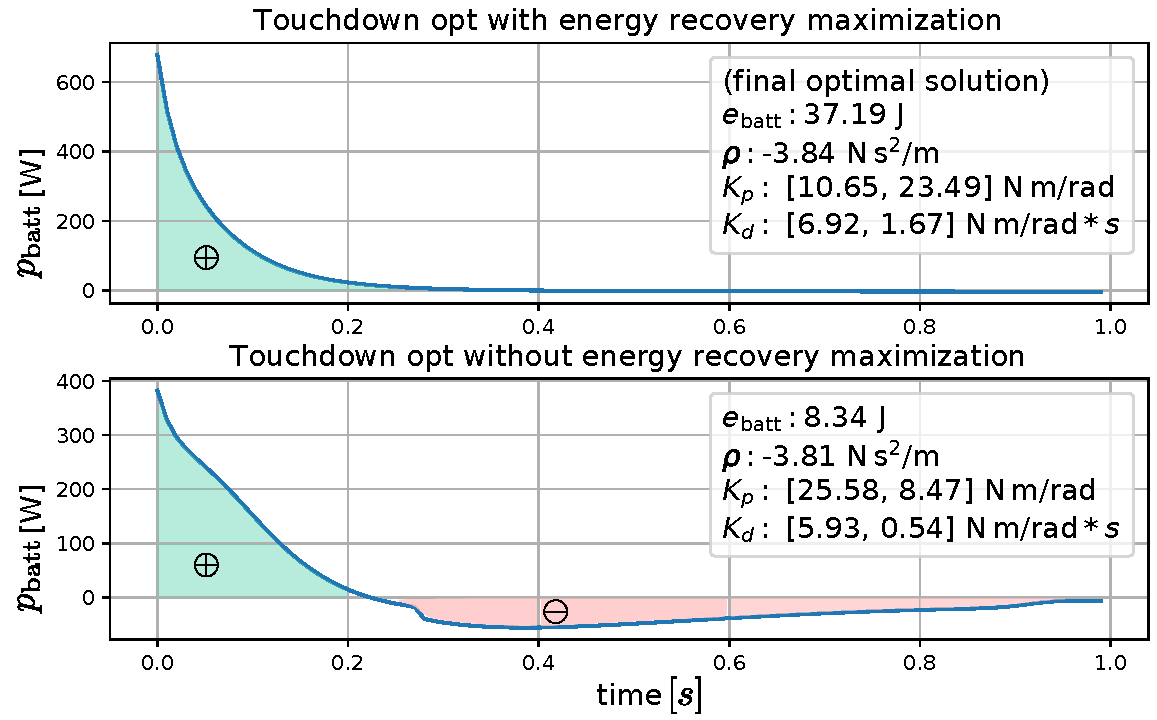
\includegraphics[width=1\columnwidth]{images/critically_damped_vs_no_reg_pow_max.pdf}
%	\caption{}
%	\label{fig:critically_damped_power}
%\end{figure}

\begin{figure}[t]
	\centering
	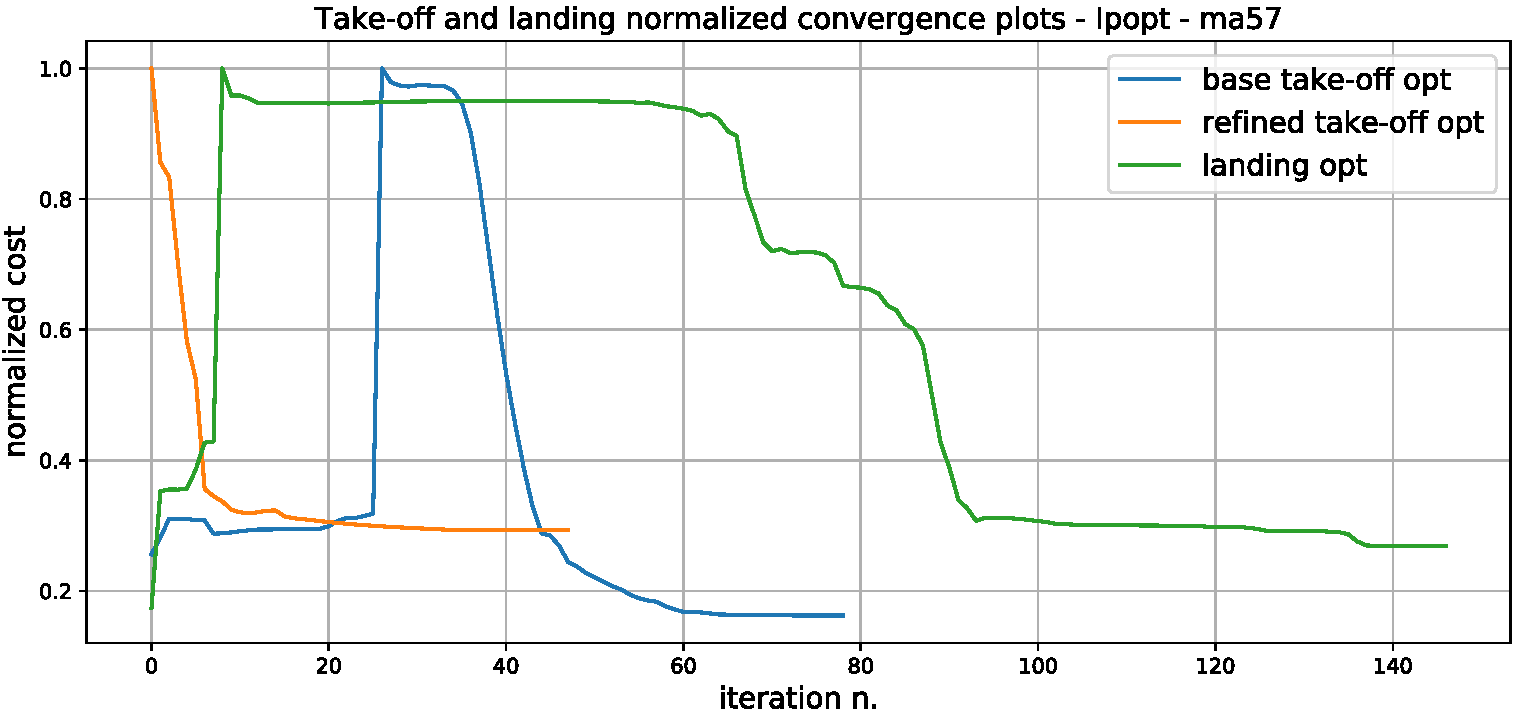
\includegraphics[width=1\columnwidth]{images/solver_conv_plots.pdf}
	\caption{Normalized convergence plots for the solution of the take-off and landing optimizations.\vspace{-0.5cm}}
	\label{fig:convergence_plots}
\end{figure}

\begin{figure}[t]
    \centering
    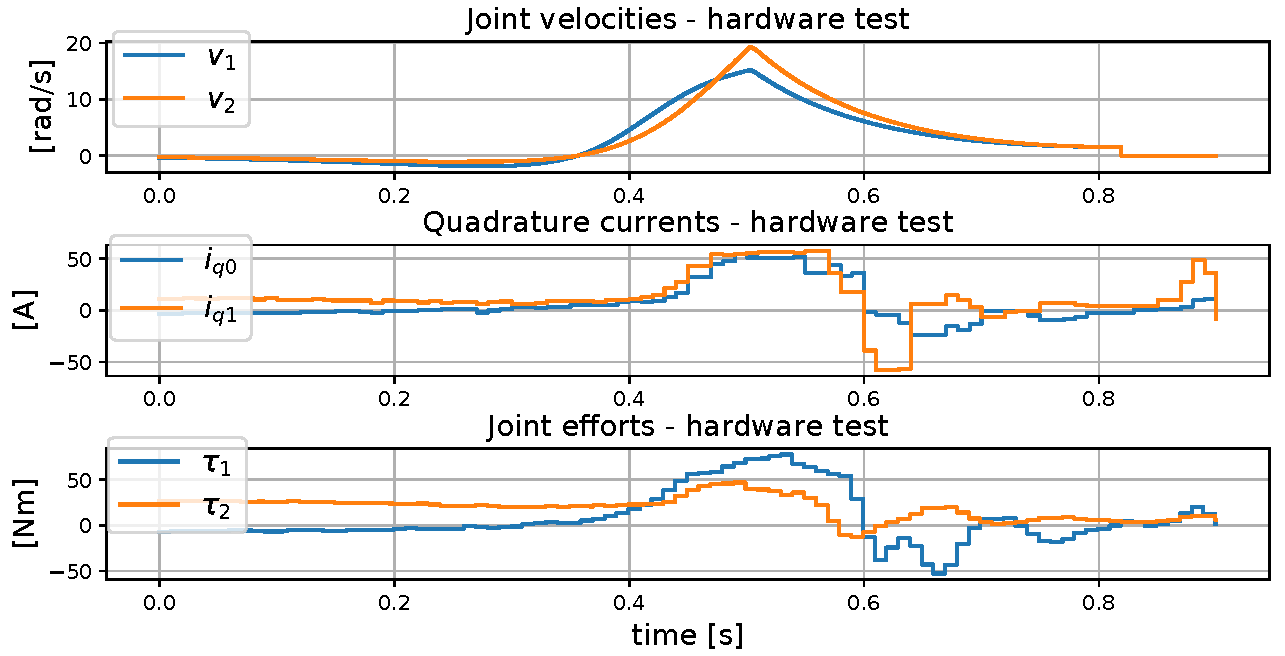
\includegraphics[width=1\columnwidth]{images/hardware_saturation.pdf}
    \caption{Data collected during the execution of the refined optimal take-off trajectory on the real robot. On top, a validation of the $i_q$ model (shown on the hip joint) during the take-off, which shows its accuracy also for highly dynamic motions. At the bottom, the measured currents (left half) and torques (right half), in line with the computed values shown in~Fig.~\ref{fig:takeoff_opt_data}~.\vspace{-0.3cm}}
    \label{fig:takeoff_execution}
\end{figure}

\subsection{Take-off execution}
The obtained take-off trajectory is replayed on the real robot exploiting the XBot2 middleware~\cite{xbot::LAURENZI2023104379} in a rt-safe control plugin running at $1\mathrm{KHz}$. employing a joint space impedance controller with high impedance setpoints. Specifically, the optimal trajectory is fed to the robot employing both position and velocity references. Figure~\ref{fig:takeoff_execution} shows the results of the execution of a single jumping trajectory on the real robot (snapshots of the leg during the execution of the experiment are visible in Fig.~\ref{fig:jumping_sequence}). The comparison with the nominal optimal solution~\ref{fig:takeoff_opt_data} reveals a good agreement in the peak currents and torques, thus confirming again the accuracy of our calibrated actuation model and the efficacy of the employed TO formulation.
\subsection{Energy regeneration results}
\begin{figure}[t]
    \centering
    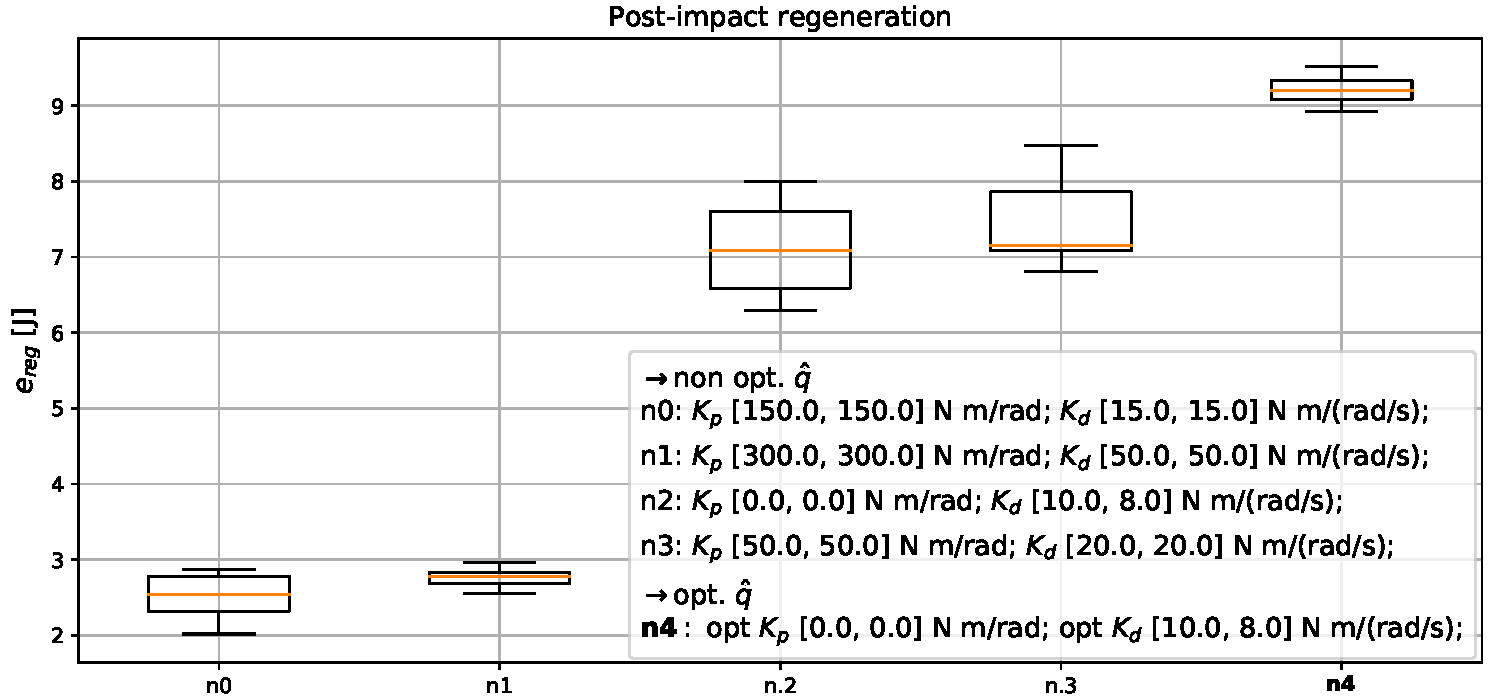
\includegraphics[width=1\columnwidth]{images/opt_vs_non_opt_conf.pdf}
    \caption{Regenerated energy at touchdown after the execution of the optimal take-off trajectory, tested on 6 impedance setpoints and landing configurations $\hat{q}$, including the optimal ones. In the non-optimal cases, the landing configuration is simply set to the one at the apex of the takeoff trajectory, i.e. $q_1~=~0.44~\mathrm{rad},~q_2~=~0.66~\mathrm{rad}$, with an associated impact ratio $\rho$~\eqref{eq:impact_ratio} of $4.65~\mathrm{N\,s^2/m}$. The optimized landing parameters~\eqref{eq:optimal_braking_sol} ($n_5$ sample) outperform all the non-optimal ones. The difference wrt the computed theoretical regeneration of $37.19~\mathrm{J}$ (see Sec.~\ref{sec:land_conf}) is attributable to the inevitable mismatches in both landing velocity and configuration generated during the pre-landing flight phase.\vspace{-0.5cm}}
    \label{fig:energy_rec_comp}
\end{figure}
In order to truly evaluate the correctness of the solution~\eqref{eq:optimal_braking_sol}, we devised a cyclic jumping test. The optimal take-off trajectory is first replayed and, while the leg is still in the air, the impedance and position reference parameters of the controller are ramped to the optimal $K_d$, $K_p$ and $\hat{q}$ given by~\eqref{eq:optimal_braking_sol}. The leg lands, we collect the estimated recovered energy, we ramp back up the impedance setpoints and then we repeat the same sequence for 15 consecutive times. Furthermore, we run again the full experiment with reasonable, but not optimized impedance setpoints, and compare the difference in the recovered energy. To avoid damages to the prototype, given the high number of jumps to be performed and the experimentally validated accuracy of~\eqref{eq:energy_flow}, we decided to execute the test only in simulation. The results are summarized in Fig.~\ref{fig:energy_rec_comp}, where we can appreciate how the optimized landing configuration and impedance combo is able to regenerate approximately $7$ times more energy that the other ones. To put these results in perspective, the dropdown tests shown in Fig.~\ref{fig:fixed_conf_reg_energy} and Fig.~\ref{fig:fixed_imp_reg_energy}, were performed by letting the leg fall from an height of $0.5\,\mathrm{m}$, which produced an impact velocity of approximately $3.16\mathrm{m/s}$, greater that the one obtained with the optimal jump. Even though the available pre-impact kinetic energy during the dropdown tests is $1.2$ times higher, the optimal solution is still able to outperform non optimized impedances and landing configurations in terms of energy recuperation.